\section{Relembrando}
\ncframesummary

\subsection*{Conceitos Básicos}
\begin{frame}{}
	\begin{block}{O que é Arduino?}
		É um projeto que engloba \textit{software} e \textit{hardware} e tem como objetivo fornecer uma plataforma fácil para prototipação de projetos interativos, utilizando um microcontrolador. O \textit{software} interage diretamente com o \textit{hardware}, tornando possível integração fácil com sensores, atuadores e outros dispositivos eletrônicos.
	\end{block}
\end{frame}

\begin{frame}{Placa Arduino Uno}
	\begin{figure}[H]
		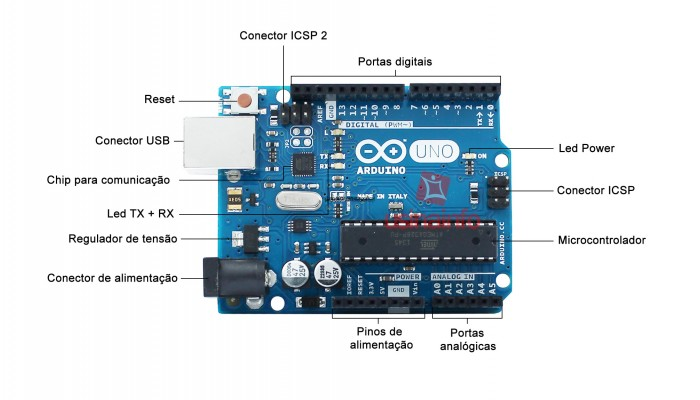
\includegraphics[width=.95\textwidth]{arduino.jpg}\footnotemark
	\end{figure}
	
	\footnotetext{http://www.usinainfo.com.br/6333-infografico/}
\end{frame}

\section{Programação Para Arduino}
\ncframesummary

\subsection*{Fundamentos}
\begin{frame}{Computador}
	\begin{block}{}
		Máquina que processa instruções. O processamento ocorre no \textbf{microprocessador}, dessa forma, entende-se que todo computador possui pelo menos um microprocessador.
	\end{block}
\end{frame}

\begin{frame}{}
	\begin{block}{}
		O Arduino utiliza um \textbf{microprocessador} do modelo ATmega. Ele pode ser \textbf{programado} para diversas funções, mas faz apenas o que está no seu \textbf{programa}. Para executar qualquer outra função ele precisa ser \textbf{reprogramado}. Por conter todos os itens básicos de um computador em um único chip, microprocessadores como o ATmega também são chamados de \textbf{microcontroladores}.
	\end{block}
\end{frame}

\begin{frame}{Programa de Computador}
	\begin{block}{}
		É uma lista de instruções para que o computador faça o que queremos.
	\end{block}
	
	\begin{figure}[H]
		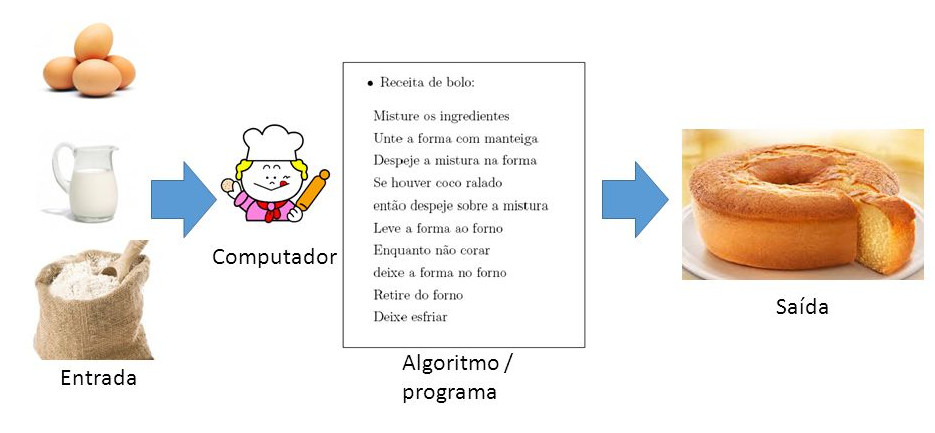
\includegraphics[width=.95\textwidth]{algoritmo.jpg}\footnotemark
	\end{figure}
	
	\footnotetext{http://slideplayer.com.br/5642541/6/images/8/}
\end{frame}

\begin{frame}{Linguagem de Máquina}
	\begin{block}{}
		Cada tipo de microprocessador entende um conjunto de instruções diferente, no seu próprio idioma, conhecido como \textbf{linguagem de máquina}. São as únicas linguagens que os computadores conseguem entender. (Alguns humanos também conseguem...)
	\end{block}
\end{frame}

\begin{frame}{Linguagem de Programação}
	\begin{block}{}
		Devido a dificuldade do ser humano em entender as linguagens de máquinas, adotamos o uso de \textbf{linguagens de programação}. Elas surgiram para que as pessoas consigam transmitir suas ideias para o computador realizar o processamento e cumprir as tarefas desejadas.  
	\end{block}
	
	\begin{figure}[H]
		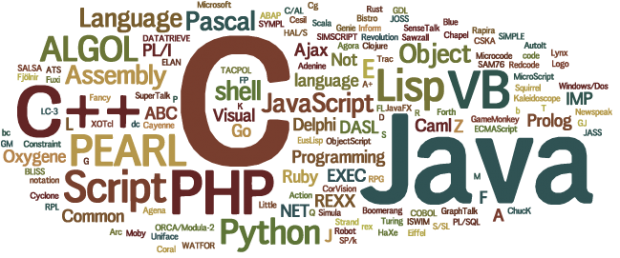
\includegraphics[width=.9\textwidth]{linguagem.png}\footnotemark
	\end{figure}
	
	\footnotetext{http://www.bosontreinamentos.com.br/wp-content/uploads/2017/05/}
\end{frame}

\begin{frame}{Compilador}
	\begin{block}{}
		Converte o programa escrito em uma \textbf{linguagem de programação} para a \textbf{linguagem de máquina}. A ação de converter o programa para a linguagem de máquina é chamada \textbf{compilar}.
	\end{block}
\end{frame}

\begin{frame}{IDE - \textit{Integrated Development Environment}}
	\begin{block}{}
		Normalmente utilizamos um \textbf{ambiente de desenvolvimento integrado} que já possui um compilador e um editor de texto onde é possível escrever o programa numa linguagem de programação específica e compilá-lo.\\
		\vspace{2 em}
		\textcolor{blue}{No caso do Arduino, a linguagem de programação adotada é C++ e o ambiente de desenvolvimento é o Arduino IDE.}
	\end{block}
\end{frame}

\begin{frame}{Código Fonte}
	\begin{block}{}
		É o nome dado ao arquivo que contém o texto do programa escrito em uma linguagem de programação.
	\end{block}
	
	\begin{figure}[H]
		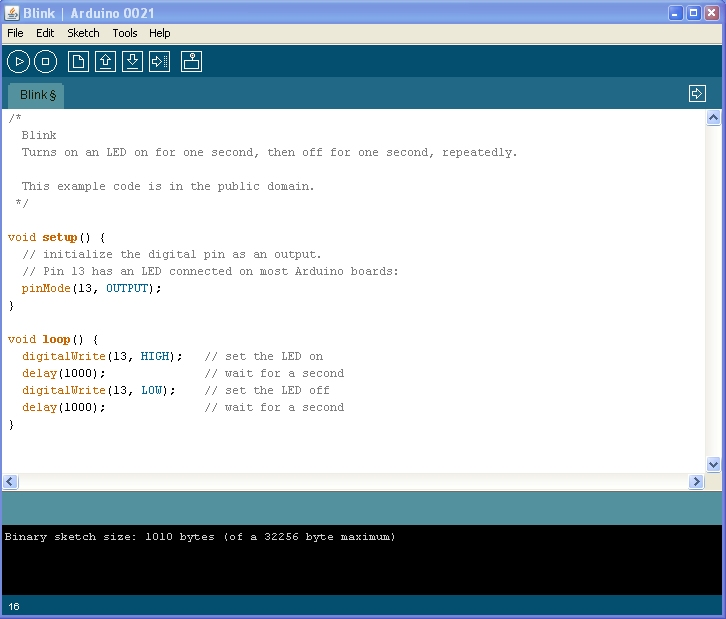
\includegraphics[width=.5\textwidth]{idefonte.jpg}\footnotemark
	\end{figure}
	
	\footnotetext{http://www.hobbytronics.co.uk/image/data/tutorial/arduino-install/}
\end{frame}

\begin{frame}{Programa/Algoritmo}
	\begin{block}{}
		É a forma de dizer para um computador o que ele deve fazer. Normalmente são escritos na forma que nós humanos entendemos, em linguagens de programação. No Arduino, um programa é conhecido como \textbf{\textit{sketch}}.
	\end{block}
\end{frame}

\subsection*{Entendendo um programa}
\begin{frame}{\textit{Blink}}
	\begin{block}{}
		Vamos analisar o programa \textit{Blink}, disponível na IDE do Arduino.
	\end{block}
	
	\centering\textbf{Veja, é uma sequência de comandos!}
	
	\lstinputlisting[language=C++, firstline=1, lastline=12]{codes/blink.cpp}
\end{frame}

\begin{frame}{Variável}
	\begin{block}{}
		Representa uma região da memória do computador (Arduino) usada para armazenar uma determinada informação\footnotemark.
	\end{block}
	
	\vspace{2em}
	\centering\textbf{Para usar uma variável no programa declara-se a variável abaixo:}
	
	\lstinputlisting[language=C++, firstline=1, lastline=1]{codes/blink.cpp}
	
	\begin{block}{}
		Nesse caso a variável declarada é do tipo \textcolor{blue}{int} e recebeu o nome de \textcolor{blue}{led}
	\end{block}
	
	\footnotetext{Pode ser um número, um caracter ou uma sequência de texto.}
\end{frame}

\begin{frame}{Tipo de Dado}
	\begin{block}{}
		Significa o tipo de informação que se pode armazenar na variável.
	\end{block}
	
	\vspace{1em}
	\centering\textbf{No arduino, os tipos de dados mais comuns são:}
	\vspace{1em}
		
	\begin{figure}[H]
		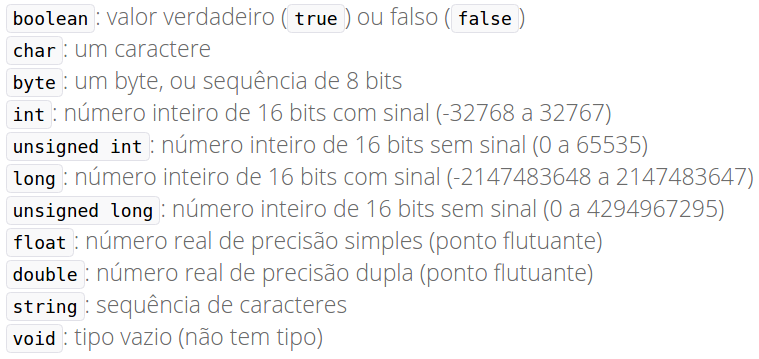
\includegraphics[width=.8\textwidth]{tiposdados.png}\footnotemark
	\end{figure}
	
	\footnotetext{https://www.circuitar.com.br/tutoriais/programacao-para-arduino-primeiros-passos/}
\end{frame}

\begin{frame}{Atribuição}
	\begin{block}{}
		Significa armazenar o valor na variável para usar posteriormente. O comando de atribuição em C++ é o =		
	\end{block}
	
	\vspace{1em}
	\centering\textbf{No exemplo, o valor 13 é atribuído à variável \textcolor{blue}{led}:}
	\vspace{1em}
	
	\lstinputlisting[language=C++, firstline=1, lastline=1]{codes/blink.cpp}
	
	\begin{block}{}
		O pino 13 do Arduino será utilizado para acender o LED, e armazenar essa informação para usar depois, ao longo do programa.
		
		Os \textbf{valores fixos} usados no programa, como o valor 13 acima, são chamados de \textbf{constantes}, pois, diferentemente das variáveis, o seu valor não muda.		
	\end{block}
\end{frame}

\begin{frame}{Função}
	\begin{block}{}
		É uma sequência de comandos que pode ser reutilizada várias vezes ao longo de um programa. 
		Fazemos uma declaração de função para criar e dizer o que ela faz.
	\end{block}
	
	\centering\textbf{Declarando uma função:}
	
	\lstinputlisting[language=C++, firstline=3, lastline=5]{codes/blink.cpp}
	
	\begin{block}{}
		A função declarada chamada \textcolor{blue}{setup()\footnotemark} executa os comando de outra função, chamada \textcolor{blue}{pinMode()} (declarada automaticamente no arduino).
	\end{block}
	
	\footnotetext{Chamada uma vez só e depois é chamada a função loop() repetidamente até que o arduino seja desligado ou reiniciado.}
\end{frame}

\begin{frame}{Parâmetros e Retorno}
	\begin{block}{Parâmetros}
		Servem para enviar algum dado para a função quando ela é chamada.
	\end{block}
	
	\begin{block}{Valor de Retorno}
		A palavra chave que vem antes do nome da função na declaração define o tipo do valor de retorno da função. Toda vez que uma função é chamada, ela é executada e devolve ou retorna um determinado valor.
	\end{block}
\end{frame}

\begin{frame}{Comentário}
	\begin{block}{}
		Trecho de texto no seu programa que serve apenas para explicar o código, sem executar nenhum tipo de comando no programa.
	\end{block}
	
	Na linguagem C++, um comentário pode ser escrito de duas formas:
	\begin{itemize}
		\item \textbf{Comentário de linha:} inicia-se com os caracteres // e deixa todo o resto da linha atual comentada.
		\item \textbf{Comentário de bloco:} inicia-se com os caracteres /* e termina com os caracteres */. Todo o texto entre o início e o término se torna um comentário, pode ser composto de várias linhas.
	\end{itemize}
\end{frame}

\begin{frame}{Exemplo}
	\lstinputlisting[language=C++, firstline=1, lastline=10]{codes/blinkcomentado.cpp}
\end{frame}

\begin{frame}{Exemplo (cont.)}
	\lstinputlisting[language=C++, firstline=11, lastline=20]{codes/blinkcomentado.cpp}
\end{frame}

\begin{frame}{Exemplo (cont.)}
	\lstinputlisting[language=C++, firstline=21, lastline=31]{codes/blinkcomentado.cpp}
\end{frame}

\begin{frame}{Estruturas de Controle (Repetição)}
	\begin{block}{}
		São blocos de instruções que alteram o fluxo de execução do código de um programa. Elas permitem que sejam executados comandos diferentes, conforme uma \textbf{condição} ou \textbf{repetir} comandos várias vezes.
	\end{block}
	
	\begin{itemize}
		\item A estrutura \textcolor{blue}{while} executa um conjunto de comandos repetidas vezes enquanto uma determinada condição for verdadeira.
		\item  A estrutura \textcolor{blue}{for} nada mais é do que um \textcolor{blue}{while} acrescido de um comando de inicialização e um comando de finalização.
	\end{itemize}
	
	\begin{figure}[ht!]
		\centering
		\subfloat[Formato do while.]
		{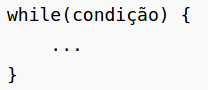
\includegraphics[width=.3\linewidth]{while.png}}
		\hfill
		\subfloat[Formado do for.]
		{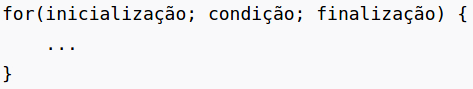
\includegraphics[width=.65\linewidth]{for.png}}
	\end{figure}
\end{frame}

\begin{frame}{Exemplo while}
	\lstinputlisting[language=C++, firstline=1, lastline=13]{codes/while.cpp}
\end{frame}

\begin{frame}{Exemplo for}
	\lstinputlisting[language=C++, firstline=1, lastline=10]{codes/for.cpp}
\end{frame}

\begin{frame}{Estruturas de Controle (Decisão)}		
	\begin{itemize}
		\item A estrutura \textcolor{blue}{if} significa "se"~em inglês. Ela verifica uma expressão e, \textbf{apenas se ela for verdadeira}, executa o conjunto de comandos.
		\item  A estrutura \textcolor{blue}{if-esle} é uma extensão do comando \textcolor{blue}{if}. \textcolor{blue}{Else} em inglês significa "caso contrário". "\textbf{Se} isso for verdadeiro, então faça aquilo, \textbf{caso contrário}, faça outra coisa".
	\end{itemize}
	
	\begin{figure}[ht!]
		\centering
		\subfloat[Formato do if.]
		{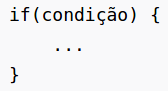
\includegraphics[width=.3\linewidth]{if.png}}
		\hfil
		\subfloat[Formado do if-else.]
		{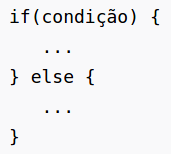
\includegraphics[width=.3\linewidth]{ifelse.png}}
	\end{figure}
\end{frame}

\begin{frame}{Exemplo if}
	\lstinputlisting[language=C++, firstline=1, lastline=7]{codes/if.cpp}
\end{frame}

\begin{frame}{Exemplo if (cont.)}
	\lstinputlisting[language=C++, firstline=8, lastline=12]{codes/if.cpp}
\end{frame}

\begin{frame}{Exemplo if-else}
	\lstinputlisting[language=C++, firstline=1, lastline=8]{codes/ifelse.cpp}
\end{frame}

\begin{frame}{Exemplo if-else (cont.)}
	\lstinputlisting[language=C++, firstline=9, lastline=16]{codes/ifelse.cpp}
\end{frame}

\section{Resumo da Aula}
\subsection*{Considerações Finais}
\begin{frame}{O que aprendemos hoje?}
	\begin{itemize}
		\item O \textcolor{blue}{arduino} é um pequeno computador, que por sua vez é um \textcolor{blue}{microprocessador} capaz de realizar o processamento de apenas um programa por vez, sendo também conhecido como \textcolor{blue}{microcontrolador};
		\item Ainda não é possível conversar com o arduino em linguagem natural, por isso escrevemos um \textcolor{blue}{programa} com o queremos que ele faça em uma \textcolor{blue}{IDE} utilizando a \textcolor{blue}{linguagem de programação} C++ para que o \textcolor{blue}{compilador} do arduino transforme as instruções contidas no \textcolor{blue}{código fonte} em \textcolor{blue}{linguagem de máquina};
		\item As linguagens de programação, no geral são compostas de \textcolor{blue}{variáveis, tipos de dados, funções e estruturas} que nos permitem dizer exatamente o que queremos que o computador faça e possibilita ao computador "entender"~o que queremos.
	\end{itemize}
\end{frame}

\section{Atividades}
\begin{frame}{Preparar o Ambiente de desenvolvimento para Arduino}
	\begin{enumerate}
		\item \textbf{Baixar e instalar o \textit{software} \textcolor{blue}{Arduino IDE} no seu computador:}
		\begin{itemize}
			\item \textbf{Onde baixar:} https://www.arduino.cc/en/Main/Software
			\item \textbf{Como instalar (Windows, Linux e MAC):} http://renatoaloi.blogspot.com.br/2011/10/instalando-arduino-guia-completo.html
		\end{itemize}
		
		\item \textbf{Baixar e instalar o \textit{software} \textcolor{blue}{fritzing} no seu computador:}
		\begin{itemize}
			\item \textbf{Onde baixar:} http://fritzing.org/download/
			\item \textbf{Como instalar (Windows, Linux e MAC):} http://fritzing.org/download/ 
		\end{itemize}
	\end{enumerate}
\end{frame}